%\documentclass[envcountsect,handout]{beamer}
\documentclass[envcountsect]{beamer}
%\setbeamertemplate{theorems}[numbered]
\usetheme{Boadilla}
% Tikz graphics
\usepackage{tikz}
\usetikzlibrary{calc, matrix, positioning}

\newtheorem{assumption}{Assumption}

\newcommand{\n}{\textbf{N}}
\renewcommand{\v}{\textbf{V}}
\renewcommand{\d}{\textbf{D}}

\newcommand{\yhat}{\hat{Y}}
\newcommand{\boldX}{X}
\newcommand{\boldY}{Y}
\newcommand{\ptheta}{p_\theta}
% Citations
\usepackage[style = authoryear]{biblatex}
\addbibresource{bibliography.bib}

\usepackage{mathtools}
\DeclareMathOperator*{\argmax}{arg\,max}

\title{Introduction to Part-of-Speech Tagging}
\subtitle{A Graphical Model for Sequence Labelling}
\author{Alex Simcock}
\institute{University of Birmingham}
\date{}

\begin{document}

\begin{frame}
\titlepage
\end{frame}

\begin{frame}{Part-of-Speech Tagging}

\begin{definition}[Part-of-Speech]
The term `part-of-speech' refers to the syntactic category of a word, for example noun, verb or adjective.
\end{definition}

\begin{example}[Ambiguous Parts-of-Speech]
\begin{center}
\begin{tabular}{ c c c c c }
 `The & fans & watch & the & race' \\
 \hline
 \textbf{Dt} & \textbf{Nn} & \textbf{Nn} & \textbf{Dt} & \textbf{Nn} \\  
 & \textbf{Vb} & \textbf{Vb} & & \textbf{Vb}    
\end{tabular}
\end{center}
\end{example}

How can we best label any given word sequence in the presence of grammatical-ambiguity?

%Part-of-speech tagging is a key preliminary step in many natural language processing pipelines.

\end{frame}

\begin{frame}

\begin{definition}[POS Tagging as Structure Prediction]

Let $\boldX$ and $\boldY$ be random variables such that $\boldX$ varies over all word sequences and $\boldY$ over all label sequences.
\begin{align*}
    \boldX &= (x_k)_{t=1}^T = (\text{`the'}, \text{`fans'}, \text{`watch'}, \text{`the'}, \text{`race'}) \\
    \boldY &= (y_k)_{t=1}^T = (\textbf{Dt}, \textbf{Nn}, \textbf{Nn}, \textbf{Dt}, \textbf{Nn}),
\end{align*}
where $y_t \in \mathcal{Y}, |\mathcal{Y}|=N$.

The POS tagging problem can now be written:

`\textbf{Given $\boldX$, predict the correctly matched tag sequence $\boldY$}'.

\end{definition}

\pause

\textbf{Maximum likelihood estimation} tells us that the best choice of $\boldY$ will maximise the probability of observing our word sequence:
\begin{equation*}
    \yhat \coloneqq \argmax_{\boldY} p(\boldY \mid \boldX).
\end{equation*}    

\end{frame}

\begin{frame}
\begin{assumption}[Independence of Observations]
    The probability of each word $x_t$ depends exclusively on the corresponding tag $y_t$ and is independent of all other elements in either sequence:
    \begin{equation*}
        p(\boldX \mid \boldY) = \prod_{t=1}^T p(x_t \mid y_t).
    \end{equation*}
\end{assumption}

\pause

\begin{assumption}[Markov Assumption]
    The probability of each tag $y_t$ is dependent (only) on its predecessor $y_{t-1}$:
    \begin{equation*}
        p(\boldY) = \prod_{t=1}^T p(y_t \mid y_{t-1}).
    \end{equation*}
\end{assumption}
%stochastic process
\end{frame}

\begin{frame}{The Hidden Markov Model (HMM)}

\begin{figure}[ht]
\centering
%\hspace{-1.9cm}
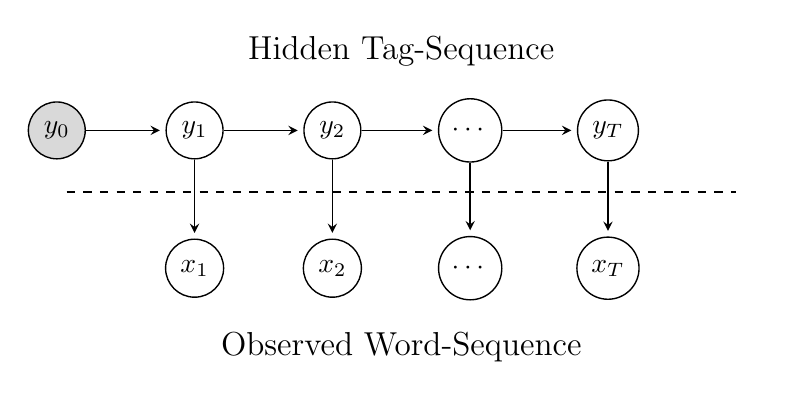
\begin{tikzpicture} [-> , >= stealth, shorten >= 2 pt, line width = 0.5pt, node distance = 1.75cm]

\node [draw, circle] (y1) {$y_1$};
\node (start) [draw, circle, fill=gray!30!white, left of = y1] {$y_0$};
\node [draw, circle] (y2) [right of = y1] {$y_2$};
\node [draw, circle] (ydot) [right of = y2] {$\cdots$};
\node [draw, circle] (yn) [right of = ydot] {$y_T$};

\path (start) edge (y1);
\path (y1) edge (y2);
\path (y2) edge (ydot);
\path (ydot) edge (yn);

\node [draw, circle] (x1) [below of = y1] {$x_1$};
\node [draw, circle] (x2) [below of = y2] {$x_2$};
\node [draw, circle] (xdot) [below of = ydot] {$\cdots$};
\node [draw, circle] (xn) [below of = yn] {$x_T$};

\path (y1) edge (x1);
\path (y2) edge (x2);
\path (ydot) edge (xdot);
\path (yn) edge (xn);


\node (c1w1) at ($(y1)!0.45!(x1)$) {};
\node (c3w3) at ($(yn)!0.45!(xn)$) {};
\draw [-, dashed, line width =0.75 pt, shorten >=-1.75cm, shorten <=-1.75cm] (c1w1) -- (c3w3);

\node (y2.5) at ($(y2)!0.5!(ydot)$) {};
\node (x2.5) at ($(x2)!0.5!(xdot)$) {};

\node [above of = y2.5, node distance= 1cm] {\large Hidden Tag-Sequence};
\node [below of = x2.5, node distance= 1cm] {\large Observed Word-Sequence};

\node (yinvis) [right of = yn] {\textcolor{white}{$y_T$}};

\end{tikzpicture}
\end{figure}

\end{frame}

\begin{frame}

The HMM can be summarised by its key parameters, the sets of emission and transition probabilities: $A$ and $B$.
\begin{align*}
    A &= [ a_{i,j} ] \quad i,j \in \mathcal{Y}, & \quad & a_{i,j} \coloneqq p(y_t = j \mid y_{t-1} = i), \\
    B  &= [ b_i(k) ] \quad i \in \mathcal{Y}, & \quad  & b_i(k) \coloneqq p(x_t = k \mid y_t = i), \\
    \pi &= [ \pi_i ] \quad i \in \mathcal{Y}, & \quad & \pi_i \coloneqq p(y_1 = i).
\end{align*}

\pause

There are three key questions for HMMs:
\begin{enumerate}
    \item Given the observed sequence $\boldX$ and a HMM $\theta = (A, B, \pi)$, how do we efficiently compute $\ptheta(\boldX) \coloneqq p(\boldX \mid \theta)$?
    \item Given the observed sequence $\boldX$ and a HMM $\theta$, how do we choose the corresponding state sequence $\boldY$ that best explains the observations?
    \item How might we adjust the model parameters in order to maximise $\ptheta(\boldX)$?
\end{enumerate}

\end{frame}

\begin{frame}

$\ptheta(\boldX)$ is also the sum of $\ptheta(\boldX, \boldY)$ over all possible state-sequences.

\begin{equation*}
    \ptheta(\boldX) = \sum_{\forall \: \boldY} \ptheta(\boldX,\boldY) = \sum_{\forall \: \boldY} \ptheta(\boldX \mid \boldY) \ptheta(\boldY)
\end{equation*}

\pause

These probabilities are given by the model assumptions:
\begin{align*}
    \ptheta(\boldX \mid \boldY) &= \prod_{t=1}^T \ptheta(x_t \mid y_t) = \prod_{t=1}^T b_{y_t}(x_t) \\
    \ptheta(\boldY) &= \prod_{t=1}^T \ptheta(y_t \mid y_{t-1}) = \pi_{y_1} \prod_{t=2}^T a_{y_{t-1},y_{t}}
\end{align*}

\pause

Hence,
\begin{equation*}
       \ptheta(\boldX) = \sum_{\forall \: \boldY} \pi_{y_1} b_{y_1}(x_1) \prod_{t=2}^T a_{y_{t-1},y_t} b_{y_t}(x_t) % a_{y_1, y_2} b_{y_2}(x_2) \cdots a_{y_{T-1}, y_T} b_{y_T}(x_T)
\end{equation*}

\pause

This calculation is \textcolor{red}{intractable} and has exponential complexity $O(2TN^T)$.
% owing to the $2n - 1$ multiplications for each of the $|\mathcal{Y}|^n$ possible values of $Y$.
% 2430 calculations with our three tags! If we had 61 tags

\end{frame}

%Prob of observations and states
\begin{frame}

    \begin{definition}[Forward-Function]
        Let $\alpha_t(i)$ denote the joint probability of observing the sequence $(x_1, x_2, \cdots, x_t)$ ($1 \leq t \leq T$) and the tag $y_t$ being $i$, given model parameters $\theta$.
        \begin{equation*}
            \alpha_t(i) \coloneqq \ptheta(x_1,x_2,\ldots,x_t,y_t=i)
        \end{equation*}
    \end{definition}

\pause

Having defined $\alpha_t(i)$, we note that $\ptheta(\boldX) = \sum_{i \in \mathcal{Y}} \alpha_T(i)$, if we can efficiently solve for a given $\alpha_t(i)$ then we have answered the first question!

\pause
\vspace{0.5cm}
\centering \textbf{Base Case:}
\begin{equation*}
        \quad \alpha_1(i) = \pi_{i} b_i(x_1) \qquad i \in \mathcal{Y}
\end{equation*}
\pause
\textbf{Inductive Step:}
\begin{equation*}
        \alpha_{t+1}(j) = \left[ \sum_{i \in \mathcal{Y}} \alpha_{t}(i)a_{i,j} \right] b_j(x_t) \qquad 
        \begin{array}{lr}
            i,j \in \mathcal{Y} \\
            1 \leq t \leq T-1
        \end{array}
\end{equation*}

\end{frame}

\begin{frame}[fragile]

\begin{figure}
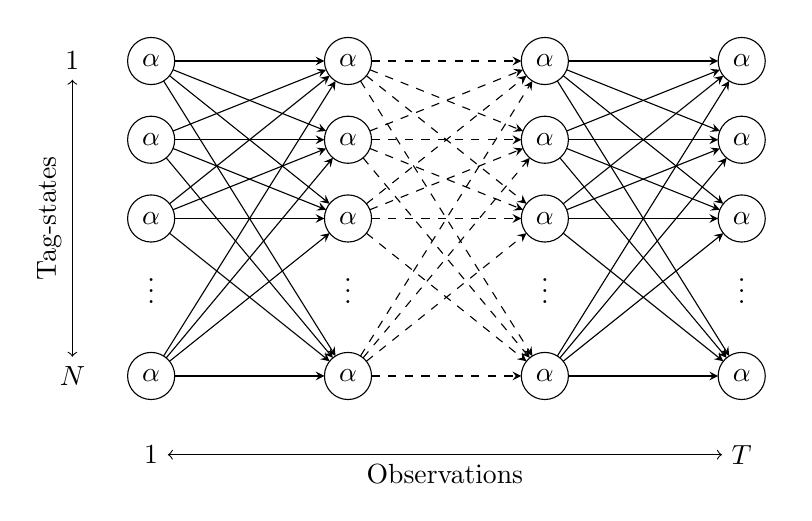
\begin{tikzpicture}
  \matrix (network)
    [matrix of nodes,%
     nodes in empty cells,
     nodes={outer sep=0pt,circle,draw},
     column sep={2.5cm,between origins},
     row sep={1cm,between origins}]
  {
    $\alpha$ & $\alpha$ & $\alpha$ & $\alpha$ \\
    $\alpha$ & $\alpha$ & $\alpha$ & $\alpha$ \\
    $\alpha$ & $\alpha$ & $\alpha$ & $\alpha$ \\
    |[draw=none]| $\vdots$ & |[draw=none]| $\vdots$ & |[draw=none]| $\vdots$ & |[draw=none]| $\vdots$ \\
    $\alpha$ & $\alpha$ & $\alpha$ & $\alpha$ \\
  };
  \foreach \x [evaluate=\x as \nextx using int(\x+1)] in {1,3}{
    \foreach \y in {1,2,3,5}{
    \foreach \i in {1,2,3,5}{
    \draw [-stealth] (network-\y-\x) -- (network-\i-\nextx);
    };
    };
    };

  \foreach \y in {1,2,3,5}{
    \foreach \i in {1,2,3,5}{
    \draw [-stealth, dashed] (network-\y-2) -- (network-\i-3);
    };
    };

    \node [below of=network-5-1] (obs1) {$1$};
    \node [below of=network-5-4] (obsT) {$T$};
    \draw[<->] (obs1) -- (obsT) node [midway, below] {Observations};

  \node [left of=network-1-1] (state1) {$1$};
  \node [left of=network-5-1] (stateY) {$N$};
  \draw[<->] (state1) -- (stateY) node [midway, left, rotate=90, anchor=base, yshift=6pt] {Tag-states};
\end{tikzpicture}
\caption{Forward-Function Calculation Trellis}
\end{figure}

\pause
This approach calculates $\ptheta(\boldX)$ with complexity $O(TN^2)$.

\end{frame}

%At each step of induction we calculate the value $\alpha_t$ for all $|\mathcal{Y}|$ states, where each is derived from $|\mathcal{Y}|$ previous states.
%Carrying out this calculation for each of the $n-1$ steps results in overall complexity of order $O(n|\mathcal{Y}|^2)$.


\begin{frame}



Given a pre-trained HMM and a set of only 10 tags we can now calculate the likelihood of generating an arbitrary 5 word sentence like `the fans watch the race' ($N=10,t=5$) with $\frac{1}{2000}$ times as many calculations.

\pause
\vspace{0.5cm}

\textbf{The British National Corpus includes 61 tags, which would correspond to a reduction in calculations of order $10^{15}$.}

\pause

\vspace{0.5cm}

$\alpha$ is only the first of several helper variables that apply the principle of dynamic programming to speed up calculations for HMMs and other, more advanced graphical methods such as the Conditional Random Field (CRF).

\pause

\vspace{0.5cm}

The algorithms for tagging and training both HMMs and CRFs are discussed in full detail in my project and I recommend the papers \textit{`A tutorial on hidden Markov models and selected applications in speech recognition'} \footcite{rabiner-1989-tutorial} and \textit{`An introduction to conditional random fields'} \footcite{sutton-2012-crfintro} for comprehensive tutorials of the mathematics behind these models.

\end{frame}

\begin{frame}
\centering \Huge
\emph{Thank you}
\end{frame}
\end{document}